\section{Signal Model}
\label{sec:model}

\begin{figure}[t]
  \centerline{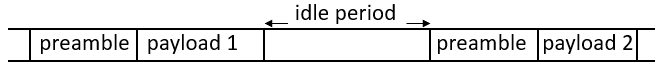
\includegraphics[width=3.4in]{data_structure.png}}
  \caption{Structure of signal stream at the receiver}
  \label{fig:data_structure}
  \end{figure}

In an uplink multiuser system, the transmitted signal frame from each user is seperated by an unkown length of idle period and assumed to include a reference signal that is known to the receiver.
Often such a reference sequence is prepended to the payload and is referred to as a preamble.
The structure of signal stream at the receiver is shown in Figure~\ref{fig:data_structure}. 
The problem addressed in this paper is to accurately estimate the start time of the preamble and to estimate carrier phase and frequency offset from the preamble.
Hence, the payload portion of the frame is not further considered. 
% Moreover, to make our algorithm applicable for signal transmission in very high speed,
% the complexity of algorithm is also crucial.

We now give the signal model for this paper. The received RF signal is first modulated at base band.
In~\cite{Morelli_Mengali_98} and~\cite{Ramakrishnan_10}, 
the authors obtain a simplifed signal model from the matched filter outputs by assuming the symbol time is perfectly known.
However, in practice, this is unreliable especially at low SNR. To accommodate this issue, we analyze the discrete signal model
directly after down-conversion and sampling, which yields received samples $r_n$

\begin{equation}
    \begin{aligned}
      \label{eq:model}
      r_n = s_{n-\bar{p}}Ae^{j\phi}e^{j2\pi\delta n}+w_{n},
    \end{aligned}
  \end{equation}
where $s_n$ denotes the sampled reference sequence (the preamble), which has the form

\begin{equation}
    \label{eq:l_ref_sig_discrete}
    s_n=\sum_{i=0}^{L_0-1} c_i g(nT_s-iT) \quad \text{for}~n=0,\ldots,N-1, 
    % \begin{dcases}
    %  \sum_{i=0}^{L_0-1} c_i g(nT_s-iT) & \text{for}~n=0,\ldots,N-1, \\
    %  0 & \text{otherwise}.
    % \end{dcases}
  \end{equation}
In~\eqref{eq:model}, $\bar{p}$ denotes the start position of the received preamble.
Note, because of the uncertainty of sampling, often the sampler may not sample exactly at the start time of the preamble, which causes
the integer delay $\bar{p}$ with a fractional delay in the range of $[-\frac{T_s}{2},\frac{T_s}{2})$, where $T_s$ is the sample period as in~\eqref{eq:l_ref_sig_discrete}.
In this paper, the sampling rate is assumed to be high enough relative to the symbol rate, so that the influence of fractional delay can be ignored.
$A$, $\phi$, $\delta$ are the amplitude, carrier phase and normalized
frequency offset with respect to sample period $T_s$ that we want to estimate.
$w_n$ is complex AWGN. Moreover,
$E_s/N_0$ denotes the ratio of signal energy to noise power spec-tral density (SNR).
To make analysis easier, we assume a con-stant and normalized envelope of the samples in the 
preamble, i.e., $A^2|s_n|^2\approx A^2=E_s/M$ for $n=[0,N-1]$, where $M$ is the rate
of oversampling in each symbol of the preamble.

In~\eqref{eq:l_ref_sig_discrete}, $T$ denotes the symbol period and $g(t)$ provides pulse shaping.
$\{c_i\}_{i=0}^{L_0-1}$ is the symbol sequence known at transmitter and receiver, where $L_0$ denotes the number of symbols.
% We further define $M$ to be the rate of oversampling in each symbol, thus $M=\frac{T}{T_s}$, and 
We define $N=ML_0$ to be the number of samples in the preamble.
Note, compared with the signal model in~\cite{Morelli_Mengali_98} and~\cite{Ramakrishnan_10}, 
by using an oversampled signal, we can mitigate the coherent loss that occurs
when the signal with frequency offset is passed through the matched filter.
This allows our system to tolerate larger frequency offsets.

% Finally, note that in~\eqref{eq:l_ref_sig_discrete}, when the discrete time index $n$ of $s_n$ is greater than $N-1$,
% or equivalently, $n>p+N-1$ in~\eqref{eq:model}, it means the received samples $r_n$ at those $n$ are in the payload;
% We assume the data of payload is zero for simplicity (normally it isn't) because it does not affect the time synchronization of the preamble and carrier synchronization from the preamble.


% The rest of paper includes two main sections. The first section (Section 3 and 4) focus on 
% analyzing the signal acquisition chain, which includes the sequential detection process and
% carrier synchronization of the preamble. The above block diagram is shown in Figure 2.
% The simulation section 5 then illustrates the performance of proposed algorithm
% in the first section. The second section (section 6) moves attention on implementing the algorithm on software-defined radio (SDR).
% Some steps (equations) in the first section are computed more efficiently to achieve the best throughput.